\section{Overview of the Project's Training Setup and Finetune Techniques}
In this section, we will introduce the organization of the source code, the training configurations of the model, and three fine-tuning techniques and implementations used in this project.

\subsection{Repository Structure Overview}

\begin{figure}[H]
    \centering
    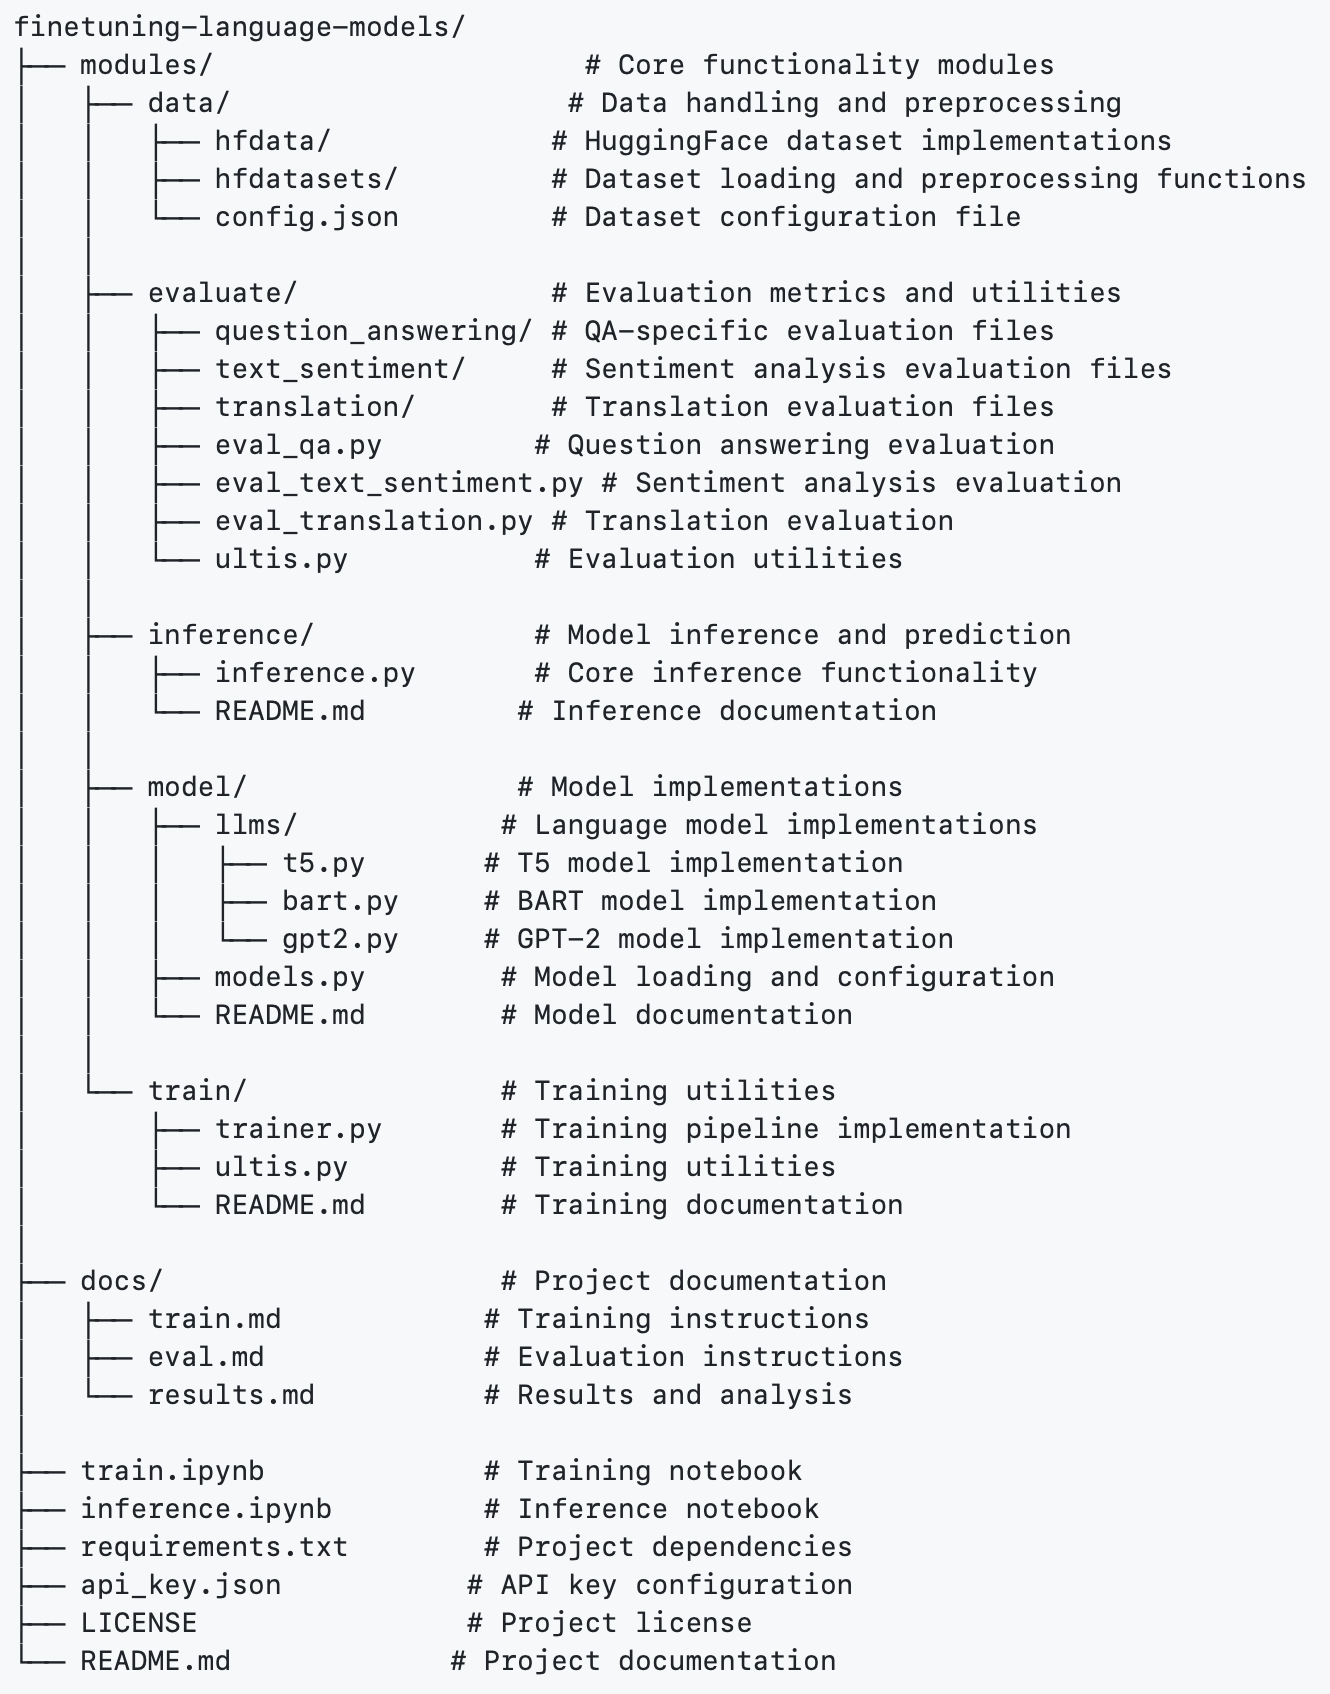
\includegraphics[width=0.95\linewidth]{img/chap06/tree.png} % Adjust width as needed
    \caption{Project structure}
    \label{fig:Tree}
\end{figure}

The repository is organized into modular folders to separate the concerns of training, evaluation, data handling, and model implementation.

\textbf{Root Files} – main source directory, organized into submodules:
\begin{itemize}
  \item \texttt{train.ipynb}: Main notebook for training language models using different fine-tuning techniques on tasks like sentiment classification, question answering, and translation.
  \item \texttt{inference.ipynb}: Used for testing pre-trained or fine-tuned models interactively.
  \item \texttt{requirements.txt}: Lists Python dependencies, including \texttt{transformers}, \texttt{datasets}, \texttt{evaluate}, and \texttt{peft}.

    \item \texttt{api\_key.json}: API key configuration for external services.
  
\end{itemize}

\textbf{modules/} – main source directory, organized into submodules:
\begin{table}[htbp]
\centering
\caption{Core folders in \texttt{finetuning-language-models-project}}
\begin{tabularx}{\textwidth}{@{} l X X @{}}
\toprule
\textbf{Path} &
\textbf{Purpose} &
\textbf{Key files / subfolders} \\
\midrule
\texttt{data/} &
Centralised data ingestion—keeps preprocessing logic separate from training. &
\texttt{hfdata/} adapters, \texttt{hfdatasets/} custom loaders, \texttt{config.json} (task-specific hyper-parameters). \\[0.6em]

\texttt{train/} &
Training utilities; thin wrapper around the Hugging Face \texttt{Trainer} with PEFT support. &
\texttt{trainer.py} (orchestrates epochs, logging, early-stopping), \texttt{ultis.py} (seed, param count, Rich/TQDM helpers). \\[0.6em]

\texttt{model/} &
Model abstractions so different back-bones (T5, BART, GPT-2) share one interface. &
\texttt{llms/} (hand-crafted wrappers for each model), \texttt{models.py} (factory for selecting the wrapper). \\[0.6em]

\texttt{evaluate/} &
Task-specific metric computation; evaluation decoupled from training. &
\texttt{eval\_qa.py}, \texttt{eval\_translation.py}, \texttt{eval\_text\_sentiment.py}, plus subfolders with JSON predictions and aggregated results. \\[0.6em]

\texttt{inference/} &
Lightweight prediction entry-point for notebooks or CLI deployment. &
\texttt{inference.py} (load checkpoint, tokenize, generate, detokenize). \\
\bottomrule
\end{tabularx}
\end{table}


\textbf{docs/} – contains Markdown documentation for training steps, inference instructions, and experimental results.

\subsection{Experimental setup}
\subsubsection{High-level Workflow}

\begin{figure}[H]
    \centering
    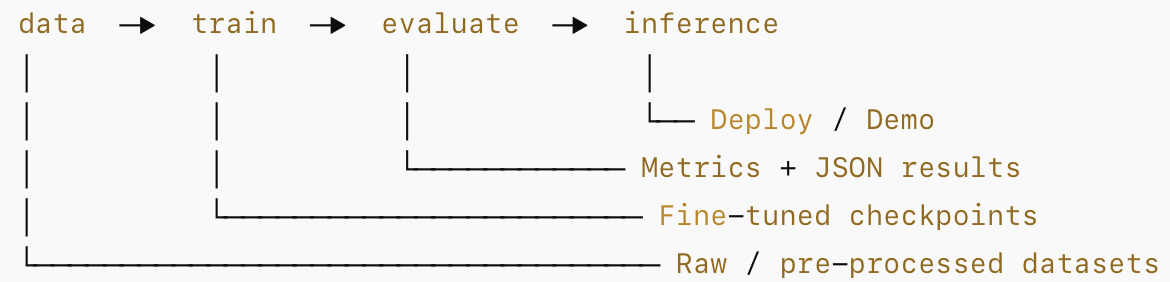
\includegraphics[width=0.95\linewidth]{img/chap06/workflow.png} % Adjust width as needed
    \caption{Workflow}
    \label{fig:Tree}
\end{figure}

\begin{table}[htbp]
\centering
\caption{Stage responsibilities in the workflow}\vspace{0.4em}
\begin{tabularx}{\textwidth}{@{} l X @{}}
\toprule
\textbf{Stage} & \textbf{What it does} \\
\midrule
\textbf{data} &
\begin{itemize}
  \item Download or collect raw corpora
  \item Clean and tokenize
  \item Wrap in a Hugging Face \texttt{DatasetDict}
\end{itemize} \\

\textbf{train} &
\begin{itemize}
  \item Load the tokenised datasets
  \item Fine-tune a backbone (Full, LoRA, Adapter)
  \item Save the \emph{best} checkpoint
\end{itemize} \\

\textbf{evaluate} &
\begin{itemize}
  \item Run the checkpoint on held-out splits
  \item Compute task metrics (BLEU, EM, F1, accuracy)
  \item Aggregate results into Markdown/JSON
\end{itemize} \\

\textbf{inference} &
\begin{itemize}
  \item Load the validated checkpoint
  \item Offer CLI / notebook / API endpoints
\end{itemize} \\
\bottomrule
\end{tabularx}
\end{table}

\newpage

\subsubsection{Environment setup}

\textbf{Prerequisites} - To run the project, the following are required:
\begin{itemize}
\item Python 3.8 or higher
\item Git
\item CUDA-compatible GPU (recommended)
\end{itemize}

\textbf{Recommended Hardware:}\\
We recommend using an NVIDIA T4 GPU or better. The T4 provides 16GB VRAM and supports FP16 training, offering a good trade-off between performance and cost. In addition, there are some alternative options including
\begin{itemize}
\item \textbf{RTX 3060 / 3060 Ti}: 12GB VRAM, affordable and supports mixed precision
\item \textbf{GTX 1080 Ti}: Older but still useful with 11GB VRAM (no native FP16 support)
\item \textbf{RTX 2060 Super / 2070}: Reasonable performance for small/medium model fine-tuning
\item \textbf{Laptop GPUs (e.g., RTX 4050/4060 Mobile)}: Suitable for lightweight experimentation with small batch sizes
\end{itemize}
\textbf{Cloud Platforms:}
We can use these platforms to run the model:
\begin{itemize}
\item \textbf{Kaggle:} Free access to T4 GPUs (30h/week), easy notebook interface, and dataset integration.
\item \textbf{Google Colab:} Similar to Kaggle, with free limited GPU hours.
\item \textbf{AWS SageMaker:} Pay-as-you-go GPU instances with more control.
\item \textbf{Google Cloud Platform:} Variety of GPU options; requires billing setup.
\end{itemize}

\textbf{Create Virtual Environment:}\\
\textbf{For Linux users,} this is what we will do:

\begin{enumerate}
\item Install Python:

\begin{lstlisting}[language=Python, caption=Download Python, basicstyle=\ttfamily\footnotesize, keywordstyle=\color{blue}]
# Ubuntu/Debian
sudo apt update
sudo apt install python3.8 python3.8-venv python3-pip

# CentOS/RHEL
sudo yum install python38 python38-devel python38-pip
\end{lstlisting}
\item Set up and activate virtual environment:
\begin{lstlisting}[language=Python, caption=Virtual env, basicstyle=\ttfamily\footnotesize, keywordstyle=\color{blue}]
# Create a new directory for your project
mkdir finetuning-language-models
cd finetuning-language-models

# Create virtual environment
python3.8 -m venv venv

# Activate virtual environment
source venv/bin/activate

# Install dependencies
pip install -r requirements.txt
\end{lstlisting}
\item Optional: Install CUDA toolkit (for GPU support only)
\begin{lstlisting}[language=Python, caption=CUDA, basicstyle=\ttfamily\footnotesize, keywordstyle=\color{blue}]
# Ubuntu/Debian
sudo apt install nvidia-cuda-toolkit

# CentOS/RHEL
sudo yum install cuda
\end{lstlisting}
\end{enumerate}


\textbf{For Window users}:

\begin{enumerate}
\item Install Python:

\begin{lstlisting}[language=Python, caption=Download Python, basicstyle=\ttfamily\footnotesize, keywordstyle=\color{blue}]
# Download and install Python 3.8+ from python.org
# During installation, check "Add Python to PATH"
\end{lstlisting}
\item Set up and activate virtual environment:
\begin{lstlisting}[language=Python, caption=Virtual env, basicstyle=\ttfamily\footnotesize, keywordstyle=\color{blue}]
# Create a new directory for your project (if not already done)
mkdir finetuning-language-models
cd finetuning-language-models

# Create virtual environment
python -m venv venv

# Activate virtual environment
.\venv\Scripts\activate

# Install dependencies
pip install -r requirements.txt
\end{lstlisting}
\item Optional: Install CUDA toolkit (for GPU support only)
\begin{lstlisting}[language=Python, caption=CUDA, basicstyle=\ttfamily\footnotesize, keywordstyle=\color{blue}]
# Reactivate environment if needed
# Windows:
.\venv\Scripts\activate
# Linux:
source venv/bin/activate
# Check Python version
python --version
# Confirm CUDA
nvidia-smi
\end{lstlisting}
\end{enumerate}

\textbf{Installation Verification}
After setting up the environment, we need to verify the installation:
\begin{lstlisting}[language=Python, caption=Verification, basicstyle=\ttfamily\footnotesize, keywordstyle=\color{blue}]
# Reactivate environment if needed
# Windows:
.\venv\Scripts\activate
# Linux:
source venv/bin/activate
# Check Python version
python --version
# Confirm CUDA
nvidia-smi
\end{lstlisting}



\subsection{Fine-Tuning Techniques}

Fine-tuning is the process of adapting a pre-trained language model to a specific task or dataset. While pre-trained models capture a general understanding of language, task-specific adaptation is necessary to maximize performance. This section presents three major techniques:

\begin{itemize}
\item \textbf{Full Fine-Tuning}: Updates all model parameters. Offers the highest performance but is computationally expensive.
\item \textbf{LoRA (Low-Rank Adaptation)}: Introduces trainable low-rank matrices into selected attention layers. Only these matrices are updated, reducing compute and memory usage.
\item \textbf{Adapter Tuning}: Inserts small trainable adapter modules between layers of the pre-trained model. The main model remains frozen.
\end{itemize}

Each method provides a trade-off between efficiency and performance, making it possible to adapt large models even on modest hardware setups. Now we will explain how these fine-tuning techniques are used in three problems: QUESTION ANSWERING, TRANSLATION, TEXT SENTIMENT.

\subsubsection{Question Answering}

\begin{lstlisting}[language=Python, caption=Full fine-tuning for QA]
#BART / T5
from transformers import AutoModelForSeq2SeqLM
model = AutoModelForSeq2SeqLM.from_pretrained(model_path)


#GPT-2
from model.llms.gpt2 import GPT2ForExtractiveQA
model = GPT2ForExtractiveQA.from_pretrained(model_path)
\end{lstlisting}
\textit{Why it fits:} Full fine-tuning is ideal for QA where precise span or text generation is needed. It enables deeper task-specific adaptation for complex reasoning.

\begin{lstlisting}[language=Python, caption=LoRA fine-tuning for QA]
from peft import LoraConfig, get_peft_model
from peft.utils.other import prepare_model_for_kbit_training

lora_config = LoraConfig(
task_type=TaskType.QUESTION_ANSWERING,
inference_mode=False,
r=32,
lora_alpha=32,
lora_dropout=0.01,
bias="none"
)

#BART

lora_config.target_modules = ["q_proj", "v_proj", "k_proj", "out_proj"]
model = AutoModelForSeq2SeqLM.from_pretrained(model_path)
model = get_peft_model(model, lora_config)

#GPT-2

lora_config.target_modules = ["attn.c_attn", "attn.c_proj", "mlp.c_proj"]
model = GPT2ForExtractiveQA.from_pretrained(model_path)
model = prepare_model_for_kbit_training(model)
model = get_peft_model(model, lora_config)

#T5

lora_config.target_modules = ["q", "k", "v"]
model = AutoModelForSeq2SeqLM.from_pretrained(model_path)
model = prepare_model_for_kbit_training(model)
model = get_peft_model(model, lora_config)
\end{lstlisting}
\textit{Why it fits:} LoRA offers lightweight updates for attention-heavy tasks like QA, optimizing performance with reduced compute.

\begin{lstlisting}[language=Python, caption=Adapter tuning for QA ]

#PrefixTuning for BART

from peft import PrefixTuningConfig, get_peft_model
peft_config = PrefixTuningConfig(
task_type=TaskType.QUESTION_ANSWERING,
inference_mode=False,
num_virtual_tokens=256,
encoder_hidden_size=model.config.d_model
)
model = AutoModelForSeq2SeqLM.from_pretrained(model_path)
model = get_peft_model(model, peft_config)

AdapterHub for GPT-2 and T5

from adapters import AutoAdapterModel
from transformers import GPT2Config, T5Config

#GPT-2

config = GPT2Config.from_pretrained(model_path)
model = AutoAdapterModel.from_pretrained(model_path, config=config)
model.add_adapter("question_answering")
model.set_active_adapters("question_answering")

#T5

config = T5Config.from_pretrained(model_path)
model = AutoAdapterModel.from_pretrained(model_path, config=config)
model.add_adapter("question_answering")
model.set_active_adapters("question_answering")
\end{lstlisting}
\textit{Why it fits:} Adapter layers specialize in task-switching. PrefixTuning enhances prompts while adapters allow QA reusability with minimal storage.

%%% Subsubsection: Text Sentiment Classification
\subsubsection{Text Sentiment Classification}

\begin{lstlisting}[language=Python, caption=Full tuning for TS]
# BART /  T5
model = AutoModelForSeq2SeqLM.from_pretrained(model_path)

# GPT2 
model = GPT2LMHeadModel.from_pretrained(model_path)
\end{lstlisting}

Full fine-tuning ensures that the LLM adapts well to sentiment nuances, which are subtle and require global model changes.

\begin{lstlisting}[language=Python, caption=LoRA tuning for TS]
# LoRA Config remains the same

# BART
model = get_peft_model(AutoModelForSeq2SeqLM.from_pretrained(model_path), lora_config)

# GPT2
model = get_peft_model(GPT2LMHeadModel.from_pretrained(model_path), lora_config)

# T5
model = get_peft_model(T5ForConditionalGeneration.from_pretrained(model_path), lora_config)
\end{lstlisting}

LoRA helps to efficiently adapt attention totional expressions without full retraining.

\begin{lstlisting}[language=Python, caption=Adapter tuning for TS]
# BART
model = get_peft_model(AutoModelForSeq2SeqLM.from_pretrained(model_path), peft_config)

# GPT2
model = AutoAdapterModel.from_pretrained(model_path)
model.add_adapter("text_sentiment_analysis")
model.set_active_adapters("text_sentiment_analysis")

# T5
model = AutoAdapterModel.from_pretrained(model_path)
model.add_adapter("text_sentiment_analysis")
model.set_active_adapters("text_sentiment_analysis")
\end{lstlisting}

Adapters work well with text sentiment due to the modularity of emotion detection and can generalize with fewer parameters.

\subsubsection{Translation}

\begin{lstlisting}[language=Python, caption=Full tuning for Translation]
# BART /  T5
model = AutoModelForSeq2SeqLM.from_pretrained(model_path)

# GPT2 
model = GPT2LMHeadModel.from_pretrained(model_path)
\end{lstlisting}

In translation, full fine-tuning aligns the entire decoder/encoder structure, which is beneficial for domain-specific terminology.

\begin{lstlisting}[language=Python, caption=LoRA tuning for Translation]
# BART
model = get_peft_model(AutoModelForSeq2SeqLM.from_pretrained(model_path), lora_config)

# GPT2
model = get_peft_model(GPT2LMHeadModel.from_pretrained(model_path), lora_config)

# T5
model = get_peft_model(AutoModelForSeq2SeqLM.from_pretrained(model_path), lora_config)
\end{lstlisting}

LoRA balances performance and efficiency, making it suitable for fine-tuning large translation models on specific language pairs.


\begin{lstlisting}[language=Python, caption=Adapter tuning for Translation]
# BART
model = get_peft_model(AutoModelForSeq2SeqLM.from_pretrained(model_path), peft_config)

# GPT2
model = AutoAdapterModel.from_pretrained(model_path)
model.add_adapter("translation")
model.set_active_adapters("translation")

# T5
model = AutoAdapterModel.from_pretrained(model_path)
model.add_adapter("translation")
model.set_active_adapters("translation")
\end{lstlisting}

Adapters isolate translation-specific knowledge into modules and avoid overwriting general capabilities of pretrained LLMs.

\subsubsection{How models and fine-tune techniques were called in the project}
In \textbf{train.ipynb}, we will initialize these parameters.

\begin{figure}[H]
    \centering
    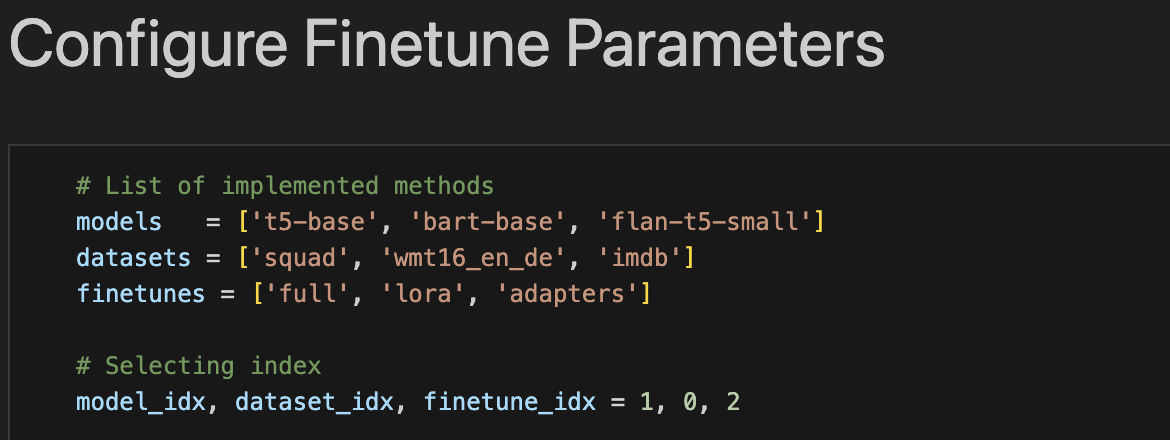
\includegraphics[width=0.95\linewidth]{img/chap06/call.png} % Adjust width as needed
    \caption{Configure finetune params}
    \label{fig:Call}
\end{figure}
This design allows quickly switching between different experiments by just changing the three indices.\\

To start the trainer, here is the code needed.
\begin{figure}[H]
    \centering
    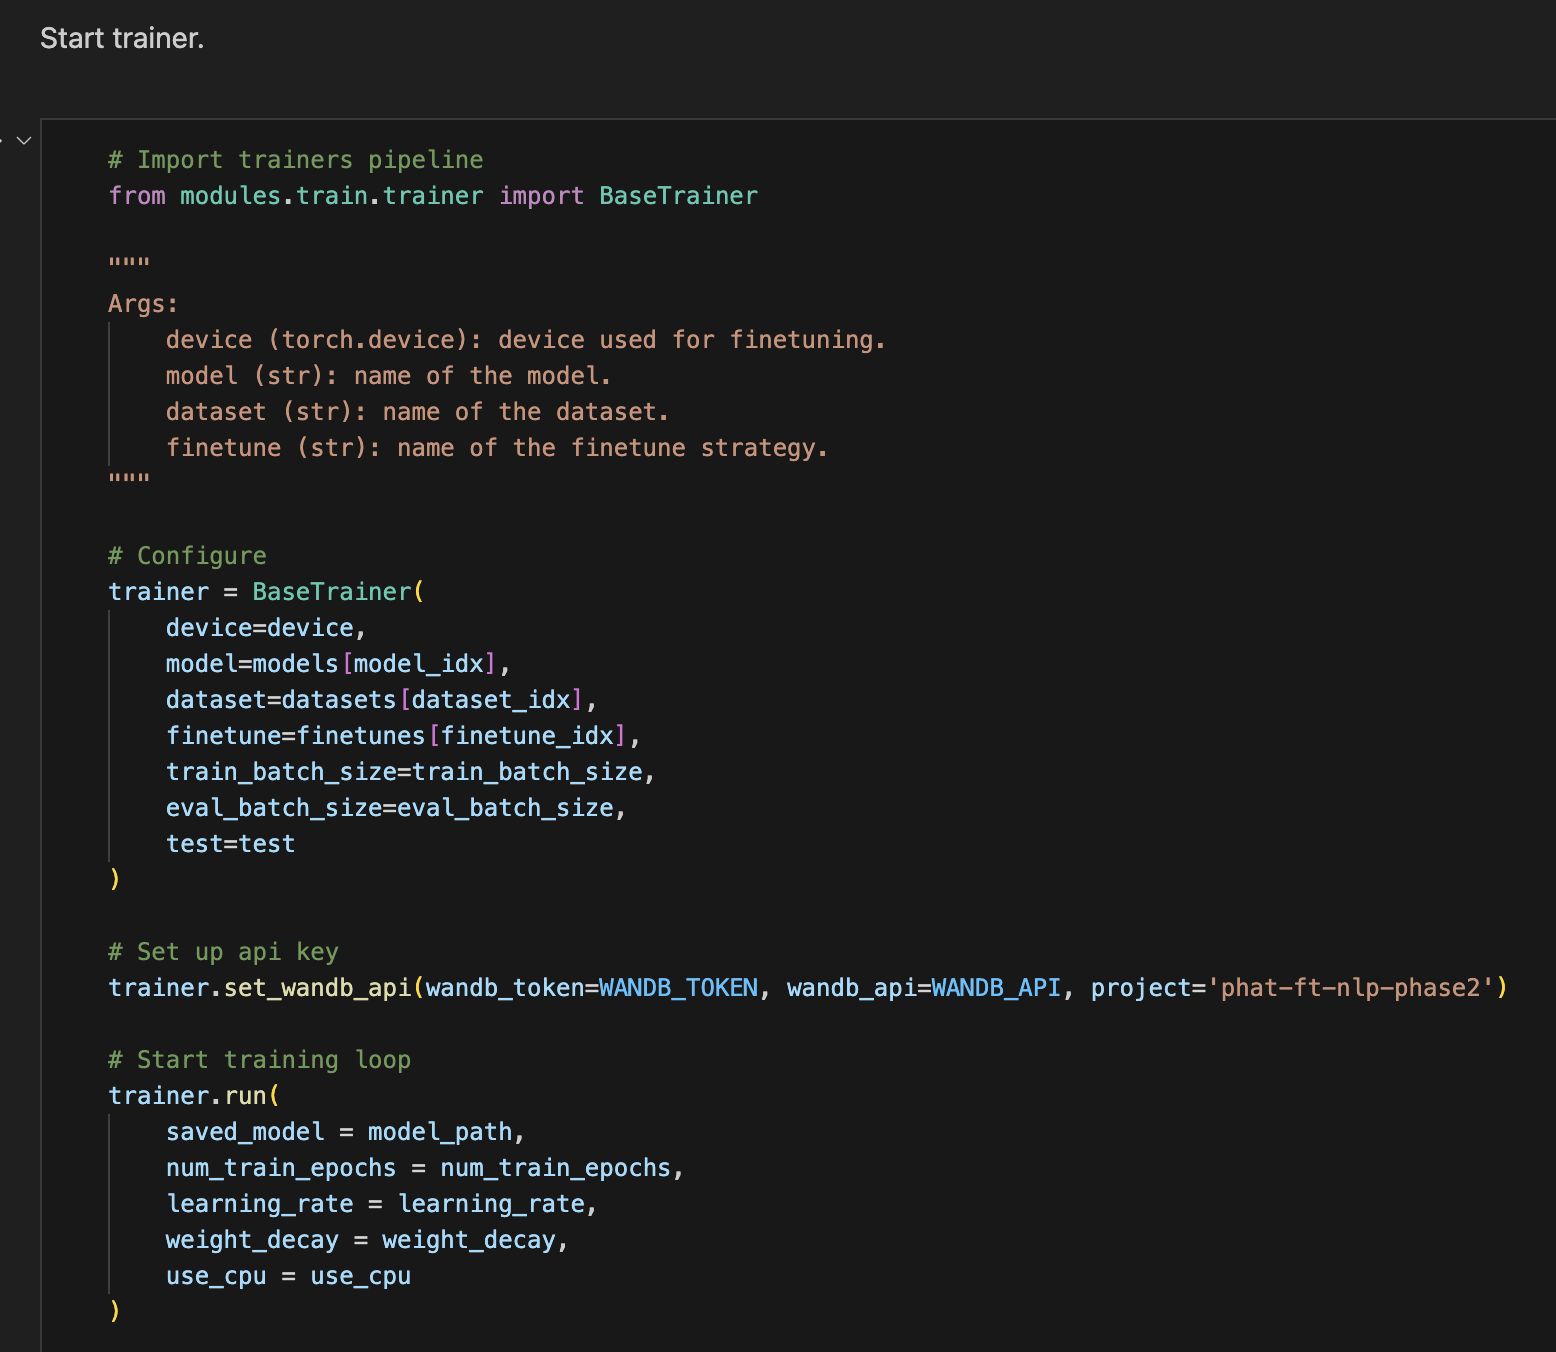
\includegraphics[width=0.95\linewidth]{img/chap06/start.png} % Adjust width as needed
    \caption{Start trainer}
    \label{fig:start}
\end{figure}

This code block serves as the final trigger that launches the fine-tuning process. It performs the following steps:

\begin{itemize}
  \item \textbf{Setup}: Initializes the training configuration, selecting the model, dataset, fine-tuning strategy, and batch sizes based on the configured indices.
  \item \textbf{Logging Integration}: Connects to Weights \& Biases (W\&B) using API credentials, allowing real-time logging of training metrics, loss curves, and checkpoints.
  \item \textbf{Execution}: Invokes the \texttt{trainer.run()} method to start the training loop, specifying the number of epochs, learning rate, weight decay, and output directory for saving the best model.
\end{itemize}

This modular design enables easy experimentation across various combinations of language models, NLP tasks, and fine-tuning techniques with minimal code changes.

